
\section{The Perceptron}

To address these concerns, \textit{\textbf{Frank Rosenblatt}} introduced the \textit{Perceptron} in 1958, funded by the U.S. Navy. Rosenblatt's model generalized the McCulloch-Pitts neuron by allowing real-valued inputs, learnable weights, and thresholds.

Formally, the perceptron computes a weighted sum of its inputs and applies a threshold to determine the binary output.
\[
y =
\begin{cases}
1 & \text{if } \sum_{i=1}^{n} w_i x_i - \theta \geq 0 \\
0 & \text{if } \sum_{i=1}^{n} w_i x_i - \theta < 0
\end{cases}
\]

A more commonly used convention rewrites this using a \textit{bias} term.
\[
y =
\begin{cases}
1 & \text{if } \sum_{i=0}^{n} w_i x_i \geq 0 \\
0 & \text{if } \sum_{i=0}^{n} w_i x_i < 0
\end{cases}
\quad \text{where } x_0 = 1 \text{ and } w_0 = -\theta
\]

This formulation shows that a perceptron still divides the input space into two halves. Inputs that produce an output of 1 lie on one side of the decision boundary $\sum w_i x_i = 0$, while those producing 0 lie on the other. 

In other words, a single perceptron can only model linearly separable functions. However, it differs from the McCulloch-Pitts model in two significant ways: the weights (including the threshold) are learnable from data, and the inputs can be real-valued.

Let us revisit the Boolean OR function. For inputs $x_1, x_2 \in \{0,1\}$, we desire an output $y = x_1 \lor x_2$. The perceptron should satisfy the following inequalities. 

\begin{table}[h]
\centering
\begin{tabular}{ccccl}
$\mathbf{x_1}$ & $\mathbf{x_2}$ & \textbf{OR} & \textbf{Inequality} & \textbf{Condition} \\
\hline
0 & 0 & 0 & $w_0 + w_1 \cdot 0 + w_2 \cdot 0 < 0$ & $\Rightarrow w_0 < 0$ \\
1 & 0 & 1 & $w_0 + w_1 \cdot 1 + w_2 \cdot 0 \geq 0$ & $\Rightarrow w_1 \geq -w_0$ \\
0 & 1 & 1 & $w_0 + w_1 \cdot 0 + w_2 \cdot 1 \geq 0$ & $\Rightarrow w_2 \geq -w_0$ \\
1 & 1 & 1 & $w_0 + w_1 \cdot 1 + w_2 \cdot 1 \geq 0$ & $\Rightarrow w_1 + w_2 \geq -w_0$
\end{tabular}
\caption{Linear inequalities that represent the OR gate using weights $w_0$, $w_1$, and $w_2$}
\end{table}


One possible solution satisfying all the above constraints is
\(
w_0 = -1, \text{ } w_1 = 1.1, \text{ and } w_2 = 1.1. 
\)

Note that this is not a unique solution—many combinations of weights satisfy the inequalities. The key insight is that for linearly separable functions like OR, a perceptron can find suitable weights to model the function accurately. We will later explore how these weights can be learned automatically using the \textit{perceptron learning algorithm} \cite{khapra2018deeplearning}.

\subsection{Perceptron Learning Algorithm}

Imagine we want to make a binary decision of whether to watch a movie or not. Suppose we are given a list of $m$ movies, each labeled as either liked (1) or not liked (0) by a user. Each movie is represented by $n$ features, which can be either Boolean or real-valued. We assume the data is linearly separable and aim to train a perceptron to learn this classification rule. In other words, we want the perceptron to find the parameters $\mathbf{w} = [w_0, w_1, \ldots, w_n]$ that define a separating hyperplane.

We now describe the perceptron learning algorithm formally.

\begin{algobox}{Perceptron Learning Algorithm}
Let $P \gets$ set of inputs labeled $1$ \\
 Let $N \gets$ set of inputs labeled $0$ \\
 Initialize weight vector $\mathbf{w}$ randomly \\
 \textbf{while} not converged \textbf{do} \\
\hspace*{1em}  Pick a random example $\mathbf{x} \in P \cup N$ \\
\hspace*{1em}  \textbf{if} $\mathbf{x} \in P$ and $\mathbf{w}^T \mathbf{x} < 0$ \textbf{then} \\
\hspace*{2em}  $\mathbf{w} \gets \mathbf{w} + \mathbf{x}$ \\
\hspace*{1em}  \textbf{if} $\mathbf{x} \in N$ and $\mathbf{w}^T \mathbf{x} \geq 0$ \textbf{then} \\
\hspace*{2em}  $\mathbf{w} \gets \mathbf{w} - \mathbf{x}$ \\
 \textbf{end while}
\end{algobox}

The algorithm continues updating the weights until all inputs are correctly classified. \textit{But why does this work?}

To understand this, consider two vectors: the weight vector $\mathbf{w} = [w_0, w_1, \ldots, w_n]$ and an input vector $\mathbf{x} = [1, x_1, \ldots, x_n]$. The perceptron computes the dot product 
\[
\mathbf{w} \cdot \mathbf{x} = \mathbf{w}^T \mathbf{x} = \sum_{i=0}^{n} w_i x_i
\]
The classification rule can then be written as 
\[
y =
\begin{cases}
1 & \text{if } \mathbf{w}^T \mathbf{x} \geq 0 \\
0 & \text{if } \mathbf{w}^T \mathbf{x} < 0
\end{cases}
\]

Geometrically, the equation $\mathbf{w}^T \mathbf{x} = 0$ defines a hyperplane that splits the input space into two halves. Any point $\mathbf{x}$ lying on this hyperplane satisfies $\mathbf{w}^T \mathbf{x} = 0$. The weight vector $\mathbf{w}$ is orthogonal to this hyperplane, because the angle $\alpha$ between $\mathbf{w}$ and any vector $\mathbf{x}$ on the hyperplane is $90^\circ$, which implies $\cos \alpha = 0$ and hence $\mathbf{w}^T \mathbf{x} = 0$.

Now consider a point $\mathbf{x} \in P$ (positive class) such that $\mathbf{w}^T \mathbf{x} < 0$. This implies that the angle between $\mathbf{w}$ and $\mathbf{x}$ is greater than $90^\circ$, i.e., $\mathbf{x}$ lies in the wrong half-space. We wish to reduce this angle so that $\mathbf{x}$ lies in the correct half-space. Updating $\mathbf{w} \gets \mathbf{w} + \mathbf{x}$ has the following effect
\[
\mathbf{w}_{\text{new}}^T \mathbf{x} = (\mathbf{w} + \mathbf{x})^T \mathbf{x} = \mathbf{w}^T \mathbf{x} + \mathbf{x}^T \mathbf{x}
\]
Since $\mathbf{x}^T \mathbf{x} > 0$, we have $\mathbf{w}_{\text{new}}^T \mathbf{x} > \mathbf{w}^T \mathbf{x}$, which implies $\cos(\alpha_{\text{new}}) > \cos(\alpha)$ and therefore $\alpha_{\text{new}} < \alpha$. This update moves the decision boundary in the desired direction, reducing misclassification.

Similarly, for a point $\mathbf{x} \in N$ (negative class) such that $\mathbf{w}^T \mathbf{x} \geq 0$, the vector $\mathbf{x}$ lies in the wrong half-space. The angle between $\mathbf{w}$ and $\mathbf{x}$ is less than $90^\circ$. Updating $\mathbf{w} \gets \mathbf{w} - \mathbf{x}$ yields
\[
\mathbf{w}_{\text{new}}^T \mathbf{x} = (\mathbf{w} - \mathbf{x})^T \mathbf{x} = \mathbf{w}^T \mathbf{x} - \mathbf{x}^T \mathbf{x}
\]
Since $\mathbf{x}^T \mathbf{x} > 0$, this results in $\mathbf{w}_{\text{new}}^T \mathbf{x} < \mathbf{w}^T \mathbf{x}$, i.e., $\cos(\alpha_{\text{new}}) < \cos(\alpha)$ and thus $\alpha_{\text{new}} > \alpha$. The update moves the vector $\mathbf{w}$ further from $\mathbf{x}$, pushing the decision boundary away from misclassified negative points.

This geometric intuition explains why the perceptron algorithm always converges for linearly separable data. At each step, it reduces the number of misclassified points by rotating the decision boundary in the correct direction.

\begin{definition}
Two sets $P$ and $N$ of points in an $n$-dimensional space are called \textit{absolutely linearly separable} if there exist $n + 1$ real numbers $w_0, w_1, \ldots, w_n$ such that every point $(x_1, x_2, \ldots, x_n) \in P$ satisfies $\sum_{i=1}^n w_i x_i > w_0$ and every point $(x_1, x_2, \ldots, x_n) \in N$ satisfies $\sum_{i=1}^n w_i x_i < w_0$.
\end{definition}

\begin{theorem}
If the sets $P$ and $N$ are finite and linearly separable, the perceptron learning algorithm updates the weight vector $\mathbf{w}_t$ only a finite number of times. In other words, if the vectors in $P$ and $N$ are tested cyclically, a weight vector $\mathbf{w}_t$ is found after a finite number of steps $t$ which separates the two sets.
\end{theorem}

\textit{Proof.} If $\mathbf{x} \in N$, then $-\mathbf{x} \in P'$, where $P' = P \cup \{-\mathbf{x} : \mathbf{x} \in N\}$. This is because if $\mathbf{w}^T \mathbf{x} < 0$, then $\mathbf{w}^T (-\mathbf{x}) > 0$.

Hence, we can consider a unified set $P'$ where every element $\mathbf{p} \in P'$ satisfies $\mathbf{w}^T \mathbf{p} \geq 0$. Without loss of generality, normalize all vectors $\mathbf{p}$ so that $\|\mathbf{p}\| = 1$. This normalization does not affect the separating condition since $\mathbf{w}^T \mathbf{p}/\|\mathbf{p}\| \geq 0$ implies $\mathbf{w}^T \mathbf{p} \geq 0$.

Let $\mathbf{w}^*$ be the normalized ideal weight vector such that $\mathbf{w}^{*T} \mathbf{p} > 0$ for all $\mathbf{p} \in P'$. Define $\delta = \min_{\mathbf{p} \in P'} \mathbf{w}^{*T} \mathbf{p} > 0$.

Now, suppose at time $t$ we inspect point $\mathbf{p}_i \in P'$ and find $\mathbf{w}_t^T \mathbf{p}_i \leq 0$. A correction is made: \[ \mathbf{w}_{t+1} = \mathbf{w}_t + \mathbf{p}_i. \]

Let $\beta$ be the angle between $\mathbf{w}_{t+1}$ and $\mathbf{w}^*$. Then,
\[
\cos \beta = \frac{\mathbf{w}^* \cdot \mathbf{w}_{t+1}}{\|\mathbf{w}_{t+1}\|} = \frac{\mathbf{w}^* \cdot (\mathbf{w}_t + \mathbf{p}_i)}{\|\mathbf{w}_{t+1}\|} = \frac{\mathbf{w}^* \cdot \mathbf{w}_t + \mathbf{w}^* \cdot \mathbf{p}_i}{\|\mathbf{w}_{t+1}\|}.
\]
Since $\mathbf{w}^* \cdot \mathbf{p}_i \geq \delta$, we obtain
\[ \mathbf{w}^* \cdot \mathbf{w}_{t+1} \geq \mathbf{w}^* \cdot \mathbf{w}_t + \delta. \]
By induction, after $k$ corrections, we have
\[ \mathbf{w}^* \cdot \mathbf{w}_t \geq \mathbf{w}^* \cdot \mathbf{w}_0 + k\delta. \]

Now consider the squared norm of $\mathbf{w}_{t+1}$:
\[
\|\mathbf{w}_{t+1}\|^2 = \|\mathbf{w}_t + \mathbf{p}_i\|^2 = \|\mathbf{w}_t\|^2 + 2 \mathbf{w}_t \cdot \mathbf{p}_i + \|\mathbf{p}_i\|^2.
\]
Since $\mathbf{w}_t \cdot \mathbf{p}_i \leq 0$ and $\|\mathbf{p}_i\| = 1$, we get
\[ \|\mathbf{w}_{t+1}\|^2 \leq \|\mathbf{w}_t\|^2 + 1. \]
Inductively,
\[ \|\mathbf{w}_t\|^2 \leq \|\mathbf{w}_0\|^2 + k. \]

Putting everything together,
\[
\cos \beta = \frac{\mathbf{w}^* \cdot \mathbf{w}_t}{\|\mathbf{w}_t\|} \geq \frac{\mathbf{w}^* \cdot \mathbf{w}_0 + k\delta}{\sqrt{\|\mathbf{w}_0\|^2 + k}}.
\]

As $k$ increases, the numerator grows linearly, but the denominator grows as $\sqrt{k}$, so $\cos \beta$ can grow unbounded. However, since $\cos \beta \leq 1$, the number of corrections $k$ must be bounded. Therefore, the perceptron algorithm must converge after a finite number of updates.

Let's have a look back at the questions raised after McCulloch-Pitts model. 

\textit{What if the inputs are not binary but real-valued?}
The perceptron works directly with real-valued inputs, using the sign of the weighted sum $\mathbf{w}^\top \mathbf{x}$ to make decisions.

\textit{Do we always need to manually specify the threshold parameter?}
No, the threshold can be learned as a bias term $w_0$ by appending a constant $x_0 = 1$ to the input vector.

\textit{Are all inputs equally important, or should some be assigned more weight?}
Inputs can have different importance, reflected in the learned weights $\mathbf{w}$, which adjust based on the training data.

\textit{Can such a neuron model functions that are not linearly separable?}
No, a single perceptron can only separate linearly separable data. We will see soon how to handle this. 

This section was developed in 1969 by two prominent MIT scientists, \textit{\textbf{Marvin Minsky}} and \textit{\textbf{Seymour Papert}}. In their book, \textit{Perceptrons}, they critically analyzed the limitations of Rosenblatt's model. They mathematically proved the above mentioned \textit{perceptron learning algorithm} and showed that a single perceptron could not solve non-linearly separable problems, such as the simple XOR function.

Their critique wasn't wrong but the fallout was dramatic. Funding dried up. Neural networks were declared a dead end. For nearly a decade, research interest in neural models collapsed.

\subsection{Layer of Perceptrons}

\textit{How many boolean functions can you design from $n$ inputs?} $2^{2^n}$. Some of them are not linear separable. There is no general formula that tells us that. For 2 input example, there are 16 possible boolean functions, of which XOR and !XOR are not linearly separable. 

\begin{table}[h]
\centering
\begin{tabular}{cc|cccccccccccccccc}
$x_1$ & $x_2$ & $f_1$ & $f_2$ & $f_3$ & $f_4$ & $f_5$ & $f_6$ & $f_7$ & $f_8$ & $f_9$ & $f_{10}$ & $f_{11}$ & $f_{12}$ & $f_{13}$ & $f_{14}$ & $f_{15}$ & $f_{16}$ \\
\hline
0 & 0 & 0 & 0 & 0 & 0 & 0 & 0 & 0 & 0 & 1 & 1 & 1 & 1 & 1 & 1 & 1 & 1 \\
0 & 1 & 0 & 0 & 0 & 0 & 1 & 1 & 1 & 1 & 0 & 0 & 0 & 0 & 1 & 1 & 1 & 1 \\
1 & 0 & 0 & 0 & 1 & 1 & 0 & 0 & 1 & 1 & 0 & 0 & 1 & 1 & 0 & 0 & 1 & 1 \\
1 & 1 & 0 & 1 & 0 & 1 & 0 & 1 & 0 & 1 & 0 & 1 & 0 & 1 & 0 & 1 & 0 & 1 \\
\end{tabular}
\caption{Functions $f_1$ to $f_{16}$ for input combinations of $x_1$ and $x_2$}
\end{table}

\begin{figure}[h!]
\centering
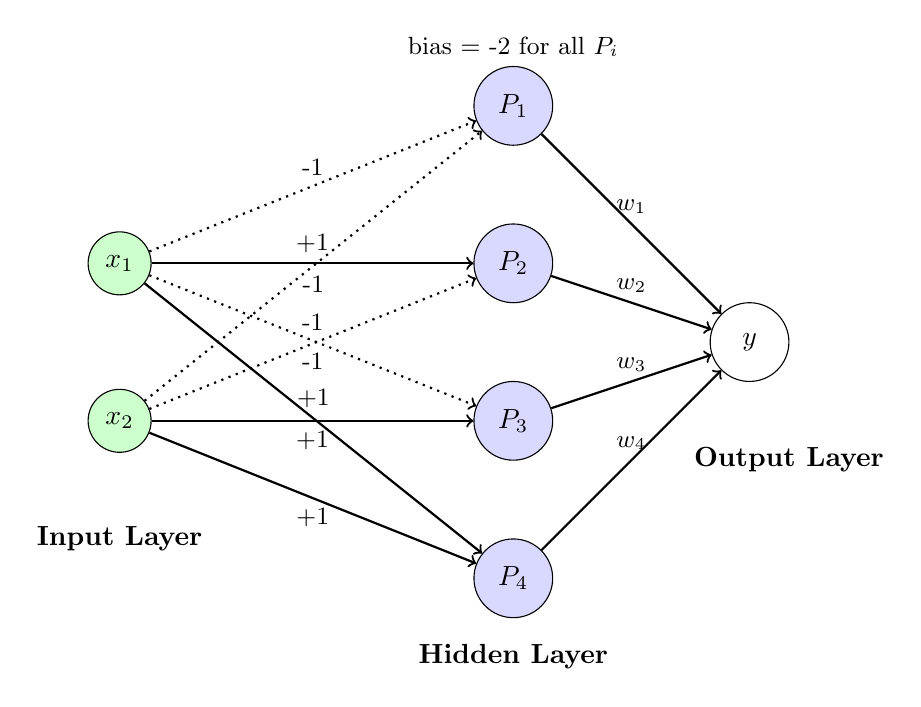
\begin{tikzpicture}[
    neuron/.style={circle, draw, minimum size=1cm, fill=blue!15},
    input/.style={circle, draw, minimum size=0.8cm, fill=green!20},
    output/.style={circle, draw, minimum size=1cm},
    weight/.style={font=\small, midway, above},
    bias/.style={font=\small, below},
    arrow/.style={->, thick},
    positive/.style={->, thick},
    negative/.style={->, thick, dotted}
]

% Input layer
\node[input] (x1) at (0, 2) {$x_1$};
\node[input] (x2) at (0, 0) {$x_2$};

% Hidden layer (4 perceptrons)
\node[neuron] (p1) at (5, 4) {$P_1$};
\node[neuron] (p2) at (5, 2) {$P_2$};
\node[neuron] (p3) at (5, 0) {$P_3$};
\node[neuron] (p4) at (5, -2) {$P_4$};

% Output layer
\node[output] (y) at (8, 1) {$y$};

% Input to hidden layer connections
\draw[negative] (x1) -- (p1) node[weight] {-1};
\draw[negative] (x2) -- (p1) node[weight, below] {-1};

\draw[positive] (x1) -- (p2) node[weight] {+1};
\draw[negative] (x2) -- (p2) node[weight, below] {-1};

\draw[negative] (x1) -- (p3) node[weight] {-1};
\draw[positive] (x2) -- (p3) node[weight, below] {+1};

\draw[positive] (x1) -- (p4) node[weight] {+1};
\draw[positive] (x2) -- (p4) node[weight, below] {+1};

% Hidden to output layer connections
\draw[arrow] (p1) -- (y) node[weight] {$w_1$};
\draw[arrow] (p2) -- (y) node[weight] {$w_2$};
\draw[arrow] (p3) -- (y) node[weight] {$w_3$};
\draw[arrow] (p4) -- (y) node[weight] {$w_4$};

% Bias annotations
\node[bias] at (5, 5) {bias = -2 for all $P_i$};

% Labels
\node at (0, -1.5) {\textbf{Input Layer}};
\node at (5, -3) {\textbf{Hidden Layer}};
\node at (8.5, -0.5) {\textbf{Output Layer}};

\end{tikzpicture}
\caption{Two Input Network with Four Hidden Perceptrons}
\end{figure}

Two binary inputs, $x_1$ and $x_2$, are passed to a hidden layer with four perceptrons $P_1$ to $P_4$. Each perceptron in the hidden layer computes a distinct linear combination of the inputs with weights $\pm1$, effectively separating different input regions. All hidden units use a fixed bias of $-2$. The outputs from the hidden layer are linearly combined in the output layer using learnable weights $w_1, w_2, w_3, w_4$ to produce the final output $y$. 

This network can implement \textit{any boolean function}, whether linearly separable or not. The key idea lies in the design of the hidden layer. Each of the four perceptrons is constructed to \textit{fire (output 1) for exactly one of the four possible input combinations} of $(x_1, x_2)$, and \textit{only} for that combination.

\begin{table}[h]
\centering
\begin{tabular}{cc}
\textbf{Perceptron} & \textbf{Input that Activates It} \\
\hline
$P_1$ & $(0, 0)$ \\
$P_2$ & $(0, 1)$ \\
$P_3$ & $(1, 0)$ \\
$P_4$ & $(1, 1)$ \\
\end{tabular}
\caption{Unique input activation for each perceptron}
\end{table}

Because each hidden unit uniquely represents one input, the output neuron can now learn the desired boolean function by \textit{assigning appropriate weights} $w_1, w_2, w_3, w_4$ to these hidden activations. For instance, to implement XOR, we can simply set the weights such that the output neuron fires for $(0,1)$ and $(1,0)$, and stays off for $(0,0)$ and $(1,1)$. This translates to the following conditions.
\[
w_1 < w_0,\quad w_2 \geq w_0,\quad w_3 \geq w_0,\quad w_4 < w_0
\]
There are \textit{no contradictions}. Thus, by adjusting the output weights accordingly, this single network architecture can represent \textit{all 16 possible boolean functions}.

\begin{theorem}
    Any boolean function of \( n \) inputs can be represented exactly by a network of perceptrons containing one hidden layer with \( 2^n \) perceptrons and one output layer containing a single perceptron \cite{khapra2018deeplearning}.
\end{theorem}

\begin{proof}
A boolean function \( f: \{0,1\}^n \to \{0,1\} \) is defined on \( 2^n \) possible input vectors.

Construct a hidden layer with \( 2^n \) perceptrons, each configured to activate only for one unique input vector by appropriate weights and bias.

The output perceptron then sums the hidden layer outputs with weights chosen to output 1 exactly for inputs where \( f \) is 1, and 0 otherwise.

Thus, the network exactly represents any boolean function.
\end{proof}

\begin{quote}
    \textbf{Note:} A network with \( 2^n + 1 \) perceptrons is not necessary but sufficient. For example, we have seen how to represent the OR function (and similarly AND function)    with just one perceptron.
\end{quote}

\begin{quote}
    \textbf{Catch:} As \( n \) increases, the number of perceptrons in the hidden layer increases exponentially.
\end{quote}